\documentclass{article}

\usepackage{natbib}
\usepackage{graphicx}
\usepackage{amsmath}
\usepackage{amssymb}
\usepackage{amsthm}
\usepackage{enumitem}
\usepackage[vlined,ruled,linesnumbered]{algorithm2e}
\renewcommand\AlCapFnt{\footnotesize}
\renewcommand\AlCapNameFnt{\footnotesize}
\renewcommand\AlFnt{\footnotesize}
\SetArgSty{textrm}
\SetKwProg{Procedure}{procedure}{}{end}
\SetKwProg{Function}{function}{}{end}
\SetKwFor{RepeatTimes}{repeat}{times do}{end}
\SetKw{Break}{break}

\usepackage{booktabs}
\usepackage{multirow}

\newtheorem{proposition}{Proposition}
\newtheorem{definition}{Definition}

\DeclareMathOperator*{\argmin}{arg\,min}
\DeclareMathOperator*{\argmax}{arg\,max}
\DeclareMathOperator*{\argsecmax}{arg\,sec\,max}

\title{Feasibility-Based Heuristic for the CPMP}


\newcommand{\mss}{s^\mathrm{src}}
\newcommand{\mds}{s^\mathrm{dst}}
\newcommand{\mts}{s^\mathrm{tmp}}


\begin{document}
\maketitle







\section{Introduction}

Since the commencement of containerization, the global use of standardized containers has dramatically improved international trade. Containers enable the smooth flow of goods between multiple transportation modes without directly handling the freight. Over the years, stringent requirements such as just-in-time operations from consignors have created additional challenges for the container transportation industry.


As one of the key components of the maritime terminals, container yards are the space dedicated to the transshipment, handover, loading, consolidation, maintenance, and storage of containers.
Some yards act as exchange venues for container transfers between different transportation modes while others are used as caches for temporary storage or as warehouses for long-term storage.

Generally, a container yard is divided into several yard blocks, each of which consists of several parallel bays. A bay is formed by a row of stacks. Usually the containers stored in the same bay have the same dimensions. Equipments such as rubber-tyre gantry cranes, rail-mounted gantry cranes, and reach stackers are frequently used in container yards. Figure \ref{cpmp:fig:block} illustrates an example of a yard block.


\begin{figure}[htbp]
\centering
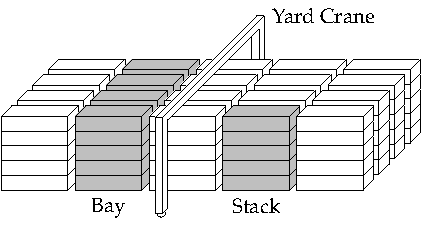
\includegraphics{figures/block.pdf}
\caption{Yard Block}
\label{cpmp:fig:block}
\end{figure}

Because containers in the same stack are organized in a LIFO (last in, first out) manner, in order to retrieve lower containers, the higher ones on the top must be  relocated first. Such forced movements are known as container reshuffles or relocations. According to recent reviews \citep{Carlo2014412,Lehnfeld2014297}, terminals deal with three major decision problems related to container reshuffling. The first problem is the selection of storage locations for arriving containers. The second is the pre-marshalling problem, which addresses the reorganization of containers inside a storage area such that no reshuffling is further required. The last problem  minimizes the total operational cost in the container retrieval process, measured by the number of relocations conducted or the total operational time. The goal of such researches on container operations is to improve terminals' performance levels, including their throughput rate per berth or the turnaround time of vessels or road trucks \citep{Kim2015}.

This chapter investigates the Container Pre-Marshalling Problem (CPMP), in which the containers within a single bay are reordered such that no subsequent reshuffling is needed. It is assumed that the retrieval order of the containers is known beforehand and that no container arrives at or leaves from the bay during pre-marshalling. In this chapter, a new concept of state feasibility is introduced. Based on that, the Feasibility-Based Heuristic is developed for solving the CPMP, which permits the freedom of selecting the next container handled not limiting to the largest priority value. This innovative heuristic strategy is a departure from the traditional one, which is the main contribution of this chapter. 

The remainder of this chapter is structured as follows. Section \ref{cpmp:sec:problem} gives a mathematical description of the CPMP, and Section \ref{cpmp:sec:literature} reviews existing approaches for solving the problem in the literature.
The Feasibility-Based Heuristic and a Beam Search algorithm are presented in Section \ref{cpmp:sec:fbh} and \ref{cpmp:sec:beam}, respectively. Section \ref{cpmp:sec:experiment} presents the numerical experiments conducted on two commonly used data sets, to examine the effectiveness of the proposed approaches. Lastly, Section \ref{cpmp:sec:conclusion} concludes this chapter and identifies future research directions.



\section{Problem Description}
\label{cpmp:sec:problem}

In the CPMP, the pre-marshalling work on a single two-dimensional bay is performed. An instance (problem input) is expressed by an initial layout of $N$ containers, which are distributed in the bay with $S$ stacks ($S\ge 3$) and $H$ tiers ($H\ge 2$), leaving $E$ empty slots ($E=SH-N$, $E\ge 2$).
In instances with $E<H$, the bottom $H-E$ tiers of the bay are unreachable. Without loss of generality, let $U=\max\{H-E,0\}$ denote the number of unreachable tiers, it is claimed that containers in the bottom $U$ tiers are immovable and the top $H-U$ tiers can be permuted into any wanted arrangement.

Let $\mathbb{S}=\{1,\dots,S\}$ denote the set of stacks. Hereafter, for simplification of description, when a stack $s$ is mentioned without declaring its value domain, it is tacitly approved that $s\in\mathbb{S}$. The height of stack $s$ is denoted by $h(s)$ and $e(s)=H-h(s)$ denotes the number of empty slots in this stack. Note that the height of stacks should not exceed $H$. The $t$-th slot (from the bottom up) of stack $s$ or the container located inside is denoted by a pair $(s,t)$. 


The containers in the bay are categorized into $P$ groups, that are determined by the particular container stowage plan based on specific constraints such as shipment destination and weight distribution. Each group is assigned a priority value from $1$ to $P$, such that a smaller priority value indicates an earlier retrieval order (earlier loading order to the container ship). The priority value of a container $c$ and that of the one located in slot $(s,t)$ are denoted by $p(c)$ and $p(s,t)$, respectively. In addition, a container with priority value $p$ is alternatively called a $p$-container for short.

To avoid confusions in presentation, hereafter we only use ``small{\slash}large priority value'' to describe a container's retrieval order, instead of ``high{\slash}low priority'' which is commonly used in the literature.

A container is orderly if it is supported directly by the ground or another orderly container with equal or larger priority value; otherwise, it is disorderly. The orderly height (i.e., number of orderly containers) of stack $s$ is denoted by $o(s)$. Other phrases referring to ``orderly{\slash}disorderly'' in the  literature include ``well{\slash}badly placed'', ``well-{\slash}non-located'', and ``clean{\slash}dirty''. 
Figure \ref{cpmp:fig:bay} demonstrates an example of a bay for which $S=5$, $H=4$, and $N=13$. Containers are represented by boxes with their priority values marked inside. In addition, boxes with gray background describe the disorderly containers.

\begin{figure}[htbp]
\centering
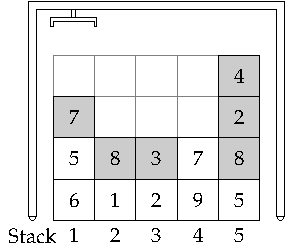
\includegraphics{figures/bay.pdf}
\caption{Bay}
\label{cpmp:fig:bay}
\end{figure}

Let us define the capability of an occupied slot $(s,t)$ by $q(s,t)=p(s,t)$ if the container inside is orderly, otherwise $q(s,t)=0$. Specifically, regarding the ground as an occupied slot at tier $0$ with capability $P$. Thus, we can easily verify the placement of a container $(s,t)$ by checking $p(s,t)\le q(s,t-1)$ (equivalently $p(s,t)=q(s,t)$).

Container orderliness is an important concept in the methodology for the CPMP, which is commonly used to measure the lower bound of a given instance. In Section \ref{cpmp:sec:stable}, a new concept called Container Stability is introduced, which is a more precise evaluation of a container's placement.

The objective of the CPMP is to find an optimized sequence with the fewest container moves capable of converting  the initial layout into a final layout in which all of the containers are orderly.

\section{Notation}

In this section, a comprehensive list of notation used in this chapter is displayed.

\newlength{\cpmpmylongest}
\settowidth{\cpmpmylongest}{$\alpha(s^+,s)$}
\addtolength{\cpmpmylongest}{\labelsep}
\SetLabelAlign{LabelCenter}{\makebox[\cpmpmylongest]{#1}}


\subsection{Global Constants}
\begin{enumerate}[noitemsep, align=LabelCenter,labelwidth=\cpmpmylongest,leftmargin=!]
\item[$N$] number of containers;
\item[$S$] number of stacks;
\item[$H$] height limitation of stacks;
\item[$P$] number of priorities;
\item[$E$] number of empty slots, $E=SH-N$;
\item[$U$] number of unreachable tiers, $U=\max\{H-E,0\}$;
\item[$\mathbb{C}$] set of containers;
\item[$\mathbb{S}$] set of stacks, $\mathbb{S}=\{1,\dots,S\}$.
\end{enumerate}

\subsection{Common Symbols and Functions}
\begin{enumerate}[noitemsep, align=LabelCenter,labelwidth=\cpmpmylongest,leftmargin=!]
\item[$L$] layout;
\item[$c$] container;
\item[$s$] stack index;
\item[$t$] tier index;
\item[$(s, t)$] slot or the container located in;
\item[$h(s)$] height of stack $s$, vectorized as $\boldsymbol{h}$;
\item[$e(s)$] number of empty slots in stack $s$, $e(s)=H-h(s)$;
\item[$o(s)$] orderly height of stack $s$, vectorized as $\boldsymbol{o}$;
\item[$f(s)$] fixed height of stack $s$, vectorized as $\boldsymbol{f}$;
\item[$p$] priority value;
\item[$p(c)$] priority value of container $c$;
\item[$p(s,t)$] priority value of container $(s,t)$;
\item[$q(s,t)$] capability of an occupied slot $(s,t)$;
\item[$(L,\boldsymbol{f})$] state;
\item[$q^f(s)$] capability of the top fixed slot in stack $s$, $q^f(s)=q(s,f(s))$.
\end{enumerate}

\subsection{Resource-{\slash}Demand-Related Functions}
\begin{enumerate}[noitemsep, align=LabelCenter,labelwidth=\cpmpmylongest,leftmargin=!]
\item[$d(p)$] order-$p$ demand, i.e., the number of unfixed $p$-containers;
\item[$D(p)$] order-$p$ accumulate demand, $D(p)=\sum_{i=p}^P d(i)$, vectorized as $\boldsymbol{D}$;
\item[$r(p)$] order-$p$ resource, $r(p)=\sum_{q^f(s)=p} (H-f(s))$;
\item[$R(p)$] order-$p$ accumulate resource, $R(p)=\sum_{i=p}^P r(i)$, vectorized as $\boldsymbol{R}$;
\item[$\Delta(p)$] order-$p$ surplus, $\Delta(p)=R(p)-D(p)$, vectorized as $\boldsymbol{\Delta}$.
\end{enumerate}

\subsection{Task-Related Symbols}
\begin{enumerate}[noitemsep, align=LabelCenter,labelwidth=\cpmpmylongest,leftmargin=!]
\item[$c^*$] target container;
\item[$s^+$] stack of the target container;
\item[$t^+$] tier of the target container;
\item[$s^-$] aim stack;
\item[$b$] number of blocking containers;
\item[$a$] number of slots available for blocking containers.
\end{enumerate}

\subsection{Extra Symbols}
\begin{enumerate}[noitemsep, align=LabelCenter,labelwidth=\cpmpmylongest,leftmargin=!]
\item[$\mss$] source stack (sender) of a move;
\item[$\mds$] destination stack (receiver) of a move;
\item[$\mts$] interim stack for temporarily storing the target container;
\item[$\vec{v}$] evaluation tuple of a move, lexicographically comparable;\item[$\mathbb{R}$] receiver set;
\item[$\mathbb{I}$] set of potential interim stacks;
\item[$\mathbb{F}$] set of potential interim stacks which are  currently full;
\item[$\mathbb{T}$] set of valid tasks.
\end{enumerate}

\subsection{Extra Functions}
\begin{enumerate}[noitemsep, align=LabelCenter,labelwidth=\cpmpmylongest,leftmargin=!]
\item[$g(s)$] stable height of stack $s$, vectorized as $\boldsymbol{ g}$;
\item[$m(s)$] messiness, the largest priority value among the unstable containers in stack $s$, $m(s)=\max_{ g(s)<t\le h(s)} p(s,t)$;
\item[$\alpha(s^+,s)$] number of slots available after the move from stack $s^+$ to $s$;
\item[$\delta(p,q)$] demand between $p$ exclusive and $q$ inclusive, $\delta(p,q)=\sum_{i=p+1}^{q}d(i)$.
\end{enumerate}

\subsection{Beam Search-Related Symbols}
\begin{enumerate}[noitemsep, align=LabelCenter,labelwidth=\cpmpmylongest,leftmargin=!]
\item[$\mathbb{B}$] set of candidate layouts in the beam;
\item[$\mathbb{O}$] set of evaluated successor layouts of the beam.
\end{enumerate}



\section{Literature Review}
\label{cpmp:sec:literature}

\subsection{Related Works}
\cite{Lee20073295} develop an integer programming model that formulates the CPMP as a multi-commodity network flow problem. The overall network is divided into several subnetworks, with each subnetwork representing an intermediate layout. The nodes in a subnetwork correspond to the slots that accommodate containers, and the commodities correspond to the containers stored in the bay. Every valid flow in the network represents a solution to the pre-marshalling problem. The model provides an innovative viewpoint to the problem, however, its performance is limited because the network is too large even for small problem instances.

\cite{Caserta2009CPMP} propose the so called corridor method for solving the problem. The method selects the direction of movement in a randomized manner according to the attractiveness of available successors confined by the corridor. The attractiveness is measured by an estimated number of additional relocations needed for the particular successor.
A local improvement procedure is also conducted to accelerate the heuristic process.


A neighborhood search approach is proposed by \cite{Lee2009468}, which repeatedly modifies the current solution until some termination condition is met. Unlike the other existing solution construction approaches, the neighborhood search is required to start from a pre-generated initial solution. 
A feasible solution can be further improved by a four-step procedure, and the diversity of the neighborhood is raised by multiple subroutines. The main drawback of the approach is the unreliability of random solution modifications, i.e., the feasibility of the resulting new solutions are not always ensured.


\cite{Bortfeldt2012CPMP} describe a tree search procedure for the pre-marshalling problem.
In the tree search structure, solutions are constructed by compound moves  instead of single moves. Moves are classified into four types, and only the most promising ones are adopted in the branching scheme.

There are two studies in the literature regarding heuristic approaches. They adopt the same heuristic strategy that containers are handled in reverse of their retrieval order.

\cite{ExpositoIzquierdo20128337} provide the first container-oriented heuristic for the CPMP, named the Lowest Priority First Heuristic. The heuristic iteratively handles containers in descending order of priority values. After handling all containers with a specific priority, a stack filling process is applied to reduce the number of disorderly containers in the bay.

\cite{Wang201567} propose the Target-Guided Heuristic for solving the problem. The Target-Guided Heuristic also handles containers in descending order of priority values. A gap utilization process is applied to enhance the heuristic performance. This work provides the first comprehensive analysis on every situation that the heuristic may face during the pre-marshalling process, especially for dense instances with fewer empty slots. In addition, the authors also develop two beam search algorithms.

\subsection{Data sets}

For examining the performance of the proposed approaches in the chapter, computational experiments are conducted on two commonly used data sets from the literature.

The first one is the CVS instances presented by \cite{Caserta2011}. The CVS instances instances are classified into 21 groups, each consisting of 40 instances. Each group is referred to as CVS $K$-$S$, where $K$ is the number of containers stacked initially in every stack and $S$ is the number of stacks of the bay. It is worth noting that the stack height limitation is not specified in the original data. Therefore, recent researchers add two extra tiers above the initial layout, that is, $H=K+2$.

The second one is the BF instances introduced by \cite{Bortfeldt2012CPMP}, which is divided into 32 groups and each group consisting of 20 instances. In the BF instances, the bay size is $S=16$ or $20$ and $H=5$ or $8$. The number of containers $N$ is either $0.6\times SH$ or $0.8\times SH$, the number of priorities $P$ is either $0.2\times N$ or $0.4\times N$, and the number of disorderly containers  $B$ is either $0.6\times N$ or $0.75\times N$ in the initial layout.



\section{Feasibility-Based Heuristic}
\label{cpmp:sec:fbh}


This section presents the Feasibility-Based Heuristic (FBH) for the CPMP\@. The main idea of this approach is to fix containers to certain stacks one by one. The order of containers handled is not limited to their priority values, which is quite different to the heuristic rules used in \citep{ExpositoIzquierdo20128337,Wang201567}.


\subsection{Main Procedure}

At every step of the FBH, the selected container and stack are referred to as the target container and the aim stack, respectively. The target container is moved to the lowest unfixed slot in the aim stack, namely the aim slot, through a sequence of moves. After that, the target container is fixed to the aim slot. Further movements on containers that have been fixed are not allowed.


A state $(L,\boldsymbol{f})$ is a pair consisting of a layout $L$ and a vector $\boldsymbol{f}$. The vector $\boldsymbol{f}$ indicates the fixed height (i.e., number of fixed containers) of each stack in the layout $L$. 
Any movements of the fixed containers are prohibited.

The heuristic first constructs the initial state according to the unreachable tiers. Starting from the initial state, the heuristic repeatedly fixes a target container $c^*$ to a properly chosen slot $(s^-,f(s^-)+1)$, until all of the containers are fixed. The overall procedure of the approach is concisely described in Algorithm \ref{cpmp:algo:overall}.

\begin{algorithm}[htbp]
\caption{Feasibility-Based Heuristic}
\label{cpmp:algo:overall}
\Begin
{
  $(L,\boldsymbol{f})\gets (L_\mathrm{init},\boldsymbol{f}_\mathrm{init})$\;
  \RepeatTimes{$N-SU$}
  {
    $(c^*, s^-)\gets \mathtt{NextTask}(L,\boldsymbol{f})$\;
    Accomplish $(c^*, s^-)$ on $L$\;
   $f(s^-)\gets f(s^-)+1$\;
  }
}
\end{algorithm}



\subsection{State Feasibility}

The fixed status of containers in a layout raises the issue of state feasibility.
In a feasible state  $(L,\boldsymbol{f})$, the following inequalities must hold: $\boldsymbol{f}\le \boldsymbol{o}$ and $\boldsymbol{\Delta}=\boldsymbol{R}-\boldsymbol{D}\ge \boldsymbol{0}$.

The former inequality indicates that only orderly containers can be fixed. 
In the latter inequality, $\boldsymbol{R}$ and $\boldsymbol{D}$ are the accumulative resource and demand vectors, and $\boldsymbol{\Delta}$ is the surplus vector. For $1\le p\le P$, $D(p)$ is the order-$p$ accumulative demand or the number of unfixed $j$-containers with $j\ge p$, and $R(p)$ is the order-$p$ accumulative resource described by the total number of slots which are able to support $p$-containers (as well as those $i$-containers with $i< p$). Introducing $d(p)$ as the number of unfixed $p$-containers and $r(p)=\sum_{q^f(s)=p} (H-f(s))$ where $q^f(s)=q(s,f(s))$, we have $D(p)=\sum_{i=p}^P d(i)$ and $R(p)=\sum_{i=p}^P r(i)$. As a result, the non-negativity of the surplus vector $\boldsymbol{\Delta}=\boldsymbol{R}-\boldsymbol{D}$ should be maintained for a feasible state.


For those states where fewer than $S-2$ stacks are fully fixed, the two inequalities are sufficient to ensure the feasibility of the state. 
Take the layout in Figure \ref{cpmp:fig:bay} as an example layout $L$ and let $\boldsymbol{f}=\boldsymbol{1}$, Table \ref{cpmp:tab:feasible} lists the computational result for the surplus vector $\boldsymbol{\Delta}$ for the example state $(L,\boldsymbol{f})$.
Observe $\Delta(7)<0$, that is to say, the containers with priority values 7, 8, and 9 cannot be well accommodated in enough unfixed slots.
As a result, the illustrated example state is infeasible.

\begin{table}[htbp]
\centering\footnotesize

\caption{Surplus Vector Computation}
\label{cpmp:tab:feasible}

\begin{tabular*}{0.5\linewidth}{c@{\extracolsep{\fill}}*5{@{}c}}
\toprule
$p$ & $d(p)$ & $D(p)$ & $r(p)$ & $R(p)$ & $\Delta(p)$ \\
\midrule
1 & 0 & 8 & 3 & 15 & 7\\
2 & 1 & 8 & 3 & 12 & 4 \\
3 & 1 & 7 & 0 & 9 & 2\\
4 & 1 & 6 & 0 & 9 & 3\\
5 & 1 & 5 & 3 & 9 & 4 \\
6 & 0 & 4 & 3 & 6 & 2\\
7 & 2 & 4 & 0 & 3 & $-1$\\
8 & 2 & 2 & 0 & 3 & 1\\
9 & 0 & 0 & 3 & 3 & 3\\
\bottomrule
\end{tabular*}
\end{table}


\begin{proposition}[Feasibility Conditions]
A state $(L,\boldsymbol{f})$ is feasible if and only if
\begin{enumerate}[label=(C\arabic*),nosep]
\item $\boldsymbol{f}\le \boldsymbol{o}$,
\item $\boldsymbol{\Delta}=\boldsymbol{R}-\boldsymbol{D}\ge \boldsymbol{0}$, and
\item fewer than $S-2$ stacks are fully fixed (i.e., $|\{s\in\mathbb{S}: f(s)=H\}|<S-2$), or
the remaining (at most two) non-fully fixed stacks can be reordered through simply transferring containers from one stack to the other.
\end{enumerate}
\end{proposition}




\subsection{Container Stability}
\label{cpmp:sec:stable}
Considering an orderly container $(s,t)$ in a feasible state $(L,\boldsymbol{f})$, we say it is stable or fixable if the resulting state by fixing $(s,t)$ and the containers below remains feasible.
Denoting the stable height (number of stable containers) of stack $s$ by $ g(s)$ (vectorized as $\boldsymbol{g}$), we will have $\boldsymbol{0}\le \boldsymbol{f}\le \boldsymbol{g}\le \boldsymbol{o}\le \boldsymbol{h}\le H\cdot\boldsymbol{1}$. If the top container of some stack, say $c$, will be stable after being moved to a non-full stack $s$, we say stack $s$ can stabilize container $c$. 

Figure \ref{cpmp:fig:stable} gives an example illustrating the stability of containers. Stable containers are marked with squares, among that back squares represent fixed containers and white squares represent stable unfixed containers. Container $(2,1)$ with priority value $6$ (marked with $\otimes$) is an orderly container but it is not stable.

\begin{figure}[htbp]
\centering
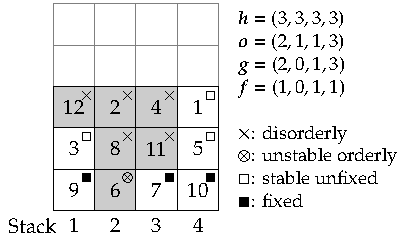
\includegraphics{figures/stable.pdf}
\caption{Stability of Containers}
\label{cpmp:fig:stable}
\end{figure}


An orderly but unstable container indicates that its orderliness is valueless because it definitely requires reshuffling.
Applying Container Stability concept is more precise with comparison to container orderliness, as an orderly but unstable container has no opportunity to be fixed to its slot.
For example, when selecting the destination stack for relocating a blocking container, the attractiveness of the destination stack candidates can be evaluated more effectively.







\subsection{Initialization}

The initial state is generated with the initial layout $L_\mathrm{init}$ and the initial fix vector $\boldsymbol{f}_\mathrm{init}=U\cdot\boldsymbol{1}$. It is a natural fact that when $S\ge 3$, containers in reachable tiers (tiers $U+1$, \dots, $H$) can be permuted into any wanted placement. Meanwhile, the bottom $U$ tiers are unreachable.
With the help of the state feasibility concept, we can check the solubility of a problem instance by checking the feasibility of the initial state. Note that the data sets tested on in this chapter are all solvable.

\subsection{Determine the Next Task}

At every step of the FBH, a task is determined through specified rules and then accomplished through a sequence of moves. A task is an assignment that aims to fix a chosen target container to the lowest unfixed slot of a chosen aim stack.
A container--stack pair $(c,s)$ is a valid task for the current state $( L,\boldsymbol{f})$ only if 
\begin{itemize}[nosep]
\item $c$ is unfixed,
\item $f(s)<H$,
\item $p(c)\le q^f(s)$, and
\item $\Delta(i)\ge H-f(s)$, for $p(c)< i\le q^f(s)$.
\end{itemize}

A valid task only guarantees the feasibility conditions C1 and C2 are satisfied, however, condition C3 is not always assured.
If a state satisfies feasibility conditions C1 and C2 but violates the last one, it is called a tricky state.
The two heuristic approaches from the literature sequentially fixes containers to chosen slots, regardless of state feasibility. In instances with less than $2(H-1)$ empty slots, there is possibility that $S-2$ stacks are fully fixed and the remaining two stacks cannot be reordered to orderliness.

There are three methods for resolving the tricky state issue.
\begin{enumerate}[nosep]
\item Prevent from entering a tricky state when deciding the next task;
\item Design an ideal task accomplishment procedure that always guarantees the resulting  state remains feasible;
\item Temporarily relocate a fixed container for completing the next task and put it back later on.
\end{enumerate}

\cite{Wang201567} adopt the last method, which yields additional moves. For dense instances where tricky states may occur, this method is far too costly.
In this chapter, the propsoed FBH adopts the first method. When selecting the next task, the FBH eliminates ``dangerous'' tasks which may lead to tricky states. This method would effectively save unnecessary moves when solving dense instances.


Besides the method that refrains from tricky states, a Bottom Tiers Protection Rule is also applied, which is motivated by the loss of the resource surplus by fixing a container.
After a target container $c$ is fixed to an aim slot $(s,f(s)+1)$, the surplus element $\Delta(i)$ is reduced by $H-f(s)$, for $p(c)< i\le q^f(s)$.
The Bottom Tiers Protection Rule balances the trade-off between the freedom of choosing the target container and the surplus loss, by eliminating the container--stack pairs $(c,s)$ such that $f(s)<2$ and $\delta(p(c),q^f(s))\ge S$, where $\delta(p,q)=\sum_{i=p+1}^{q}d(i)$. The affected demand quantity $\delta(p(c),q^f(s))$ should not reach $S$ in the bottom 2 tiers that are protected.
The number of tiers protected and the threshold value (2 and $S$ are used in this chapter) can be adjusted optionally.

Algorithm \ref{cpmp:algo:nexttask} gives the procedure of determining the next task. 
Every task $(c,s)$ in the valid task set  $\mathbb{T}$ is evaluated by function $\mathtt{EvalTask}(c,s)$. The evaluation of a valid task $(c,s)$ is a six-tuple, that starts with the key indicator, followed by the number of moves required for completing the task, the number of stable containers that need to be moved from the aim stack, the affected demand, fixed height of the aim stack, and the opposite of the target container's priority value. 
At every step of the heuristic, the next task is determined by the lexicographically minimum evaluation six-tuple. 

\begin{algorithm}[htbp]
\caption{Determine the Next Task}
\label{cpmp:algo:nexttask}

\Function{$\mathtt{NextTask}(L,\boldsymbol{f})$}
{
  $\mathbb{T}\gets \varnothing$\;
  \ForEach{$(c,s)\in\mathbb{C}\times\mathbb{S}$}
  {
      \If{$c$ is unfixed, $f(s)<H$, $p(c)\le q^f(s)$ and $\Delta(i)\ge H-f(s)$ for $p(c)< i\le q^f(s)$}
      {
        $\mathbb{T}\gets \mathbb{T}\cup\{(c,s)\}$\;
      }
  }
  \Return $\arg\min_{(c,s)\in\mathbb{T}} \mathtt{EvalTask}(c,s)$\;
}

\Function{$\mathtt{EvalTask}(c,s)$}
{
  $p\gets p(c)$, $q\gets q^f(s,f(s))$\;
  $\chi\gets 0$ \tcp*[l]{key indicator}
  \If{$|\{s\in\mathbb{S}: f(s)=H\}|=S-3$, $\sum_{s\in\mathbb{S}}f(s)<N-2$, and $f(s)=H-1$}
  {
    $\chi\gets 1$\;
  }
  \If(\tcp*[h]{Bottom Tiers Protection Rule}){$f(s)<2$ and $\delta(p,q)\ge S$}
  {
    $\chi\gets 1$\;
  }
  \Return $\langle\chi,\mathtt{MoveNeed}(c,s),g(s)-f(s),\delta(p,q),f(s),-p(c)\rangle$\;
}

\end{algorithm}


\subsection{Accomplish a Task}

After the particular task is determined by the rules described above, it is accomplished by a sequence of moves, resulting in a new state. 

\subsubsection{Preliminary}

Firstly, common functions are given in Algorithms \ref{cpmp:alg:common1} and \ref{cpmp:alg:common2}.

\begin{algorithm}[htbp]
\caption{Common Functions: Part 1}
\label{cpmp:alg:common1}

\Procedure{$\mathtt{Move}(\mss,k,\mds)$}
{
  Move $k$ containers from stack $\mss$ to stack $\mds$\;
}

 \Procedure{$\mathtt{Relocate}(\mss,k,\mathbb{R})$}
{
  \RepeatTimes{k}
  {
    $\mathbb{R}'\gets \{s\in \mathbb{R}:h(s)<H\}$\;
    $\mds\gets \argmin_{s\in\mathbb{R}'} \mathtt{EvalMove}(\mss,s)$\;
    $\mathtt{Move}(\mss,1,\mds)$\;
  }
}

\Function{$\mathtt{EvalMove}(\mss,\mds)$}
{
  $c\gets (\mss,h(\mss))$, $p\gets p(c)$, $q\gets q(\mds,h(\mds))$\;
  \uCase{$ g(\mds)=h(\mds)$ and stack $\mds$ can stabilize $c$}
  {
    \Return $\langle 1,\delta(p,q) \rangle$\;
  }
  \uCase{$ g(\mds)<h(\mds)$ and $p\ge m(\mds)$}
  {
    \Return $\langle 2,p-m(\mds) \rangle$\;
  }
  \uCase{$ g(\mds)<h(\mds)$ and $p<m(\mds)$}
  {
    \Return $\langle 3,m(\mds)-p \rangle$\;
  }
  \Case{$ g(\mds)=h(\mds)$ and stack $s_2$ cannot stabilize $c$}
  {
    \Return $\langle 4,q \rangle$\;
  }
}
\end{algorithm}

\begin{algorithm}[htbp]
\caption{Common Functions: Part 2}
\label{cpmp:alg:common2}

\Procedure{$\mathtt{BiSend}(\mss_1,k_1,\mss_2,k_2,\mathbb{R})$}
{
  $i\gets k_1$, $j\gets k_2$\;
  \RepeatTimes{$k_1+k_2$}
  {
    \uIf{$j=0$}{
      $\mathtt{Relocate}(\mss_1,i,\mathbb{R})$\;
      $i\gets 0$\;
    }
    \uElseIf{$i=0$}{
      $\mathtt{Relocate}(\mss_2,j,\mathbb{R})$\;
      $j\gets 0$\;
    }
    \Else
    {
      $\mathbb{R}'\gets \{s\in \mathbb{R}:h(s)<H\}$\;
      $\mds_1\gets \arg\min_{s\in\mathbb{R}'} \mathtt{EvalMove}(\mss_1,s)$\; $\vec{v}_1\gets \mathtt{EvalMove}(\mss_1,\mds_1)$\;
      $\mds_2\gets \arg\min_{s\in\mathbb{R}'} \mathtt{EvalMove}(\mss_2,s)$\; $\vec{v}_2\gets \mathtt{EvalMove}(\mss_2,\mds_2)$\;
      \uIf{$\vec{v}_1\le^{\mathrm{lex}} \vec{v}_2$}
      {
        $\mathtt{Move}(\mss_1,1,\mds_1)$\;
        $i\gets i-1$\;
      }
      \Else
      {
        $\mathtt{Move}(\mss_2,1,\mds_2)$\;
        $j\gets j-1$\;
      }
    }
  }
}
\Procedure{$\mathtt{BiRecv}(\mss,k_1,\mathbb{R}_1,k_2,\mathbb{R}_2)$}
{
  $i\gets k_1$, $j\gets k_2$\;
  \RepeatTimes{$k_1+k_2$}
  {
    \uIf{$j=0$}{
      $\mathtt{Relocate}(\mss,i,\mathbb{R}_1)$\;
      $i\gets 0$\;
    }
    \uElseIf{$i=0$}
    {
      $\mathtt{Relocate}(\mss,j,\mathbb{R}_2)$\;
      $j\gets 0$\;
    }
    \Else
    {
      $\mathbb{R}_1'\gets \{s\in \mathbb{R}_1:h(s)<H\}$\;
      
      
      
      $\mds_1\gets \arg\min_{s\in\mathbb{R}_1'} \mathtt{EvalMove}(\mss,s)$\; $\vec{v}_1\gets \mathtt{EvalMove}(\mss,\mds_1)$\;
      
      $\mathbb{R}_2'\gets \{s\in \mathbb{R}_2:h(s)<H\}$\;
      $\mds_2\gets \arg\min_{s\in\mathbb{R}_2'} \mathtt{EvalMove}(\mss,s)$\; $\vec{v}_2\gets \mathtt{EvalMove}(\mss,\mds_2)$\;
      
      \uIf{$\vec{v}_1\le^{\mathrm{lex}}\vec{v}_2$}
      {
        $\mathtt{Move}(\mss,\mds_1)$\;
        $i\gets i-1$\;
      }
      \Else
      {
        $\mathtt{Move}(\mss,\mds_2)$\;
        $j\gets j-1$\;
      }
    }
  }
}
\end{algorithm}




Function $\mathtt{Move}(\mss,k,\mds)$ performs $k$ relocations from stack $\mss$ to stack $\mds$. Function $\mathtt{Relocate}(\mss,k,\mathbb{R})$ performs $k$ relocations from a single sender $\mss$ to a {receiver} set $\mathbb{R}$. For each of the top $k$ containers of the sender, the destination stack $\mds$ is properly selected from $\mathbb{R}$ according to the evaluations by function $\mathtt{EvalMove}(\mss,\mds)$. The evaluations of moves are expressed as numerical tuples, which are lexicographically comparable. 

Define the messiness of stack $s$ by $m(s)=\max_{g(s)<t\le h(s)}p(s,t)$, that is the largest priority value among the unstable containers in stack $s$. The preferences of selecting a stack $\mds$ as the destination stack for a blocking container are as follows.
\begin{enumerate}[noitemsep]
\item If stack $\mds$ is entirely stable and can stabilize $c$, the minimum affected demand is preferred;
\item If stack $\mds$ is not entirely stable and $p(c)\ge m(\mds)$, the minimum gap between $m(\mds)$ and $p(c)$ is preferred;
\item If stack $\mds$ is not entirely stable and $p(c)> m(\mds)$, the minimum gap between $p(c)$ and $m(\mds)$ is preferred;
\item If stack $\mds$ is entirely stable but cannot stabilize $c$, the minimum $q(\mds,h(\mds))$ is preferred.
\end{enumerate}

The first preference indicates that stabilizing a blocking container reduces the total number of unstable containers in the bay. The second and third preferences consider the messiness of the destination stack. Messiness stands for the largest priority value of the unstable containers in a stack and larger messiness implies a higher urgency of reshuffling. The last preference indicates that an entirely stable stack should be protected from being ruined.

Function $\mathtt{BiRecv}(\mss,k_1,\mathbb{R}_1,k_2,\mathbb{R}_2)$ relocates $k_1$ and $k_2$ containers from a single sender $\mss$ to two receiver sets, $\mathbb{R}_1$ and $\mathbb{R}_2$, respectively. Similarly, function $\mathtt{BiSend}(\mss_1, k_1,  \mss_2,  k_2,  \mathbb{R})$ performs relocations from two senders, stacks $\mss_1$ and $\mss_2$, to one receiver set $\mathbb{R}$, and the respective quantities are $k_1$ and $k_2$. The moving order of the two top containers from two senders is determined by the smaller evaluation tuple.


\subsubsection{Task Types}

Let the target container be denoted by $c^*$ located in slot $(s^+,t^+)$ and the aim stack by $s^-$. The aim slot refers to the slot $(s^-,f(s^-)+1)$. The task is {immediate} if it is already located in the aim slot, {internal} if the aim slot is below the target container in the same stack, and {external} if the aim slot is in a different stack. 

\subsubsection{Immediate Task}

An immediate task does not require a move because the target container is already located in the aim slot, that is, $\mathtt{MoveNeed}(c^*,s^-)=0$ for an immediate task $(c^*,s^-)$.

\subsubsection{Internal Task}

For an internal task where $s^+=s^-$ and $t^+>f(s^+)+1$, let $a$ denote the number of empty slots in $\mathbb{S}\setminus\{s^+\}$ with the exclusion of the highest non-full stack, that is, $a=E-e(s^+)-\min\{e(s)>0: s\neq s^+\}$.  Let $b_1=h(s^+)-t^+$ and $b_2=t^+-f(s^+)-1$ denote the numbers of blocking containers above and below $c^*$ in stack $s^+$, respectively. The accomplishment procedure for an internal tack is given in  Algorithm \ref{cpmp:alg:internal}, which is divided into three cases,
\begin{itemize}[nosep]
\item I1: $a\ge b_2$;
\item I2: $a<b_2$ and $|\{s\neq s^+: h(s)<H\}|>1$; and
\item I3: $a<b_2$ and $|\{s\neq s^+: h(s)<H\}|=1$.
\end{itemize}


\begin{algorithm}[htbp]

\caption{Accomplish an Internal Task}
\label{cpmp:alg:internal}

\SetKwProg{One}{Case I1:}{}{end}
\SetKwProg{Two}{Case I2:}{}{end}
\SetKwProg{Three}{Case I3:}{}{end}


\Function{$\alpha(s^+,\mds)$}
{
  $e^{\min}\gets \min\{e(s)>0:s\neq s^+\}$\;
  $e^{\sec}\gets \min\{e(s)>e^{\min}:s\neq s^+\}$\;
  $k^{\min}\gets |\{s\neq s^+ : e(s)=e^{\min}\}|$\;
  \uIf{$e(\mds)> e^{\min}$}
  {
    \Return $E-e(s^+)-e^{\min}-1$\;
  }
  \uElseIf{$e^{\min}\ge 2$}
  {
    \Return $E-e(s^+)-e^{\min}$\;
  }
  \uElseIf{$k^{\min}=1$}
  {
     \Return $E-e(s^+)-e^{\sec}-1$\;
  }
  \Else
  {
    \Return $E-e(s^+)-2$\;
  }
}
\One{$a\ge b_2$}
  {
    \RepeatTimes{$b_1$}
    {
      
      $\mathbb{R}\gets \{s\neq s^+: h(s)<H,\, \alpha(s^+,s)\ge b_2\}$\;
      
      $\mathtt{Relocate}(s^+,1,\mathbb{R})$\;
    }
    $\mathbb{I}\gets \{s\neq s^+: h(s)<H,\, E-e(s^+)-e(s)\ge b_2\}$\;
    
    $\mts\gets \mathtt{Interim}(\mathbb{I})$\;
    $\mathtt{Move}(s^+,1,s')$\;
    $\mathtt{Relocate}(s^+,b_2,\mathbb{S}\setminus\{s^+,\mts\})$\;
    $\mathtt{Move}(\mts,1,s^+)$\;
    \tcp{I1:\ $b_1+b_2+2$ moves}
  }


  \Two{$a<b_2$ and $|\{s\neq s^+: h(s)<H\}|>1$}
  {
    $\mathtt{Relocate}(s^+, b_1, \mathbb{S}\setminus\{s^+\})$\;
    $\mts_1\gets \mathtt{Interim}(\mathbb{S}\setminus\{s^+\})$\;
    $\mathtt{Move}(s^+, 1, \mts_1)$\;
    $k_2\gets E-e(s^+)-e(\mts_1)-1$\;
    $\mathtt{Relocate}(s^+, k_2, \mathbb{S}\setminus\{s^+,\mts_1\})$\;
    Find $\mts_2\neq s^+,\mts_1$ such that $h(\mts_2)<H$\;
    $\mathtt{Move}(\mts_1, 1, \mts_2)$\;
    $\mathtt{Move}(s^+, b_2-k_2, \mts_1)$\;
    $\mathtt{Move}(\mts_2, 1, s^+)$\;
    \tcp{I2:\ $b_1+b_2+3$ moves}
  }
  
  \Three{$a<b_2$ and $|\{s\neq s^+: h(s)<H\}|=1$}
  {
    Find $s'$ such that $s'\neq s^+$ and $h(s')<H$\;
    $\mts\gets \mathtt{InterimFull}(\mathbb{S}\setminus\{s^+,s'\})$\;
    $\mathtt{BiSend}(\mts, 1, s^+, b_1, \{s'\})$\;
    $\mathtt{Move}(s^+, 1, \mts)$\;
    $\mathtt{Move}(s^+, b_2, s')$\;
    $\mathtt{Move}(\mts, 1, s^+)$\;
    \tcp{I3:\ $b_1+b_2+3$ moves}
  }
  


\end{algorithm}

In Case I1, function $\alpha(s^+,s)$ is defined similar to $a$, representing the number of empty slots in $\mathbb{S}\setminus\{s^+\}$, with the exclusion of the highest non-full stack after the topmost blocking container of stack $s^+$ is moved to stack $s$.


\subsubsection{External Task}

For an external task where $s^+\neq s^-$, the number of empty slots in $\mathbb{S}\setminus\{s^+,s^-\}$ is denoted by $a$ such that $a=E-e(s^+)-e(s^-)$. Let $b_1=h(s^+)-t^+$ and $b_2=h(s^-)-f(s^-)$ denote the numbers of blocking containers above the target container $c^*$ and the aim slot $(s^-,f(s^-))$, respectively. The pseudo-code describing the accomplishment for an external task is given in Algorithm \ref{cpmp:alg:external}, consisting of four cases,
\begin{itemize}[nosep]
\item E1: $a\ge b_1+b_2$;
\item E2: $b_1+1\le a<b_1+b_2$; 
\item E3: $1\le a<b_1+\min\{1,b_2\}$; and
\item E4: $a=0<b_1+b_2$.
\end{itemize}




\begin{algorithm}[htbp]
\caption{Accomplish an External Task}
\label{cpmp:alg:external}

\SetKwProg{One}{Case E1:}{}{end}
\SetKwProg{Two}{Case E2:}{}{end}
\SetKwProg{Three}{Case E3:}{}{end}
\SetKwProg{Four}{Case E4:}{}{end}


\One{$a\ge b_1+b_2$}
  {
    $\mathtt{BiSend}(s^+, b_1,s^-,b_2, \mathbb{S}\setminus\{s^+,s^-\})$\;
    $\mathtt{Move}(s^+, 1, s^-)$\;
    \tcp{E1:\ $b_1+b_2+1$ moves}
  }
  
\Two{$b_1+1\le a<b_1+b_2$}
  {
    $k_2\gets a-1-b_1$\;
    $\mathtt{BiSend}(s^+, b_1, s^-, k_2, \mathbb{S}\setminus\{s^+,s^-\})$\;
    Find $\mts\neq s^+,s^-$ such that $h(\mts)<H$\;
    $\mathtt{Move}(s^+,1,\mts)$\;
    $\mathtt{Move}(s^-, b_2-k_2, s^+)$\;
    $\mathtt{Move}(\mts, 1, s^-)$\;
    \tcp{E2:\ $b_1+b_2+2$ moves}
  }

\Three{$1\le a<b_1+\min\{1,b_2\}$}
  {
    $k_1\gets a-1$\;
    $\mathtt{BiRecv}(s^+, k_1, \mathbb{S}\setminus\{s^+,s^-\}, b_1-k_1, \{s^-\})$\;
    Find $\mts\neq s^+,s^-$ such that $h(\mts)<H$\;
    $\mathtt{Move}(s^+,1,\mts)$\;
    $\mathtt{Move}(s^-, b_1-k_1+b_2, s^+)$\;
    $\mathtt{Move}(\mts, 1, s^-)$\;
    \tcp{E3:\ $2b_1+b_2-a+3$ moves}
  }
  
\Four{$a=0<b_1+b_2$}
  {
    $\mts\gets \mathtt{InterimFull}(\mathbb{S}\setminus\{s^+,s^-\})$\;
    $\mathtt{BiSend}(\mts, 1, s^+, b_1, \{s^-\})$\;
    $\mathtt{Move}(s^+, 1, \mts)$\;
    $\mathtt{Move}(s^-, b_1+b_2+1, s^+)$\;
    $\mathtt{Move}(\mts, 1, s^-)$\;
    \tcp{E4:\ $2b_1+b_2+4$ moves}
  }
  
\end{algorithm}


\subsubsection{Interim Stack Selection}

In Cases I1 and I2, an interim stack is selected to temporarily store the target container. 
The selection prefers stacks that are not entirely stable, with the largest messiness, then entirely stable stacks with the smallest capability. The most unattractive stack for receiving blocking containers is selected as the interim stack. In Cases I3 and E4, the interim stack is selected by the minimum priority value of the top containers of these full stacks.

\begin{algorithm}[htbp]

\caption{Interim Stack Selection}


\Function{$\mathtt{Interim}(\mathbb{I})$}
{
  $\mathbb{I}_1\gets \{s\in \mathbb{I}: g(s)<h(s)<H\}$\;
  $\mathbb{I}_2\gets \{s\in \mathbb{I}:  g(s)=h(s)<H\}$\;
  
  \uIf{$\mathbb{I}_1\neq \varnothing$}
  {
    \Return $\argmax_{s\in\mathbb{I}_1} m(s)$\;
  }
  \Else
  {
    \Return $\argmin_{s\in\mathbb{I}_2} q(s,h(s))$\;
  }
}




\Function{$\mathtt{InterimFull}(\mathbb{F})$}
{
  $\mathbb{F}_1\gets \{s\in \mathbb{F}: f(s)\le g(s)<h(s)=H \}$\;
  $\mathbb{F}_2\gets \{s\in \mathbb{F}: f(s)< g(s)=h(s)=H \}$\;
  \tcp{it is guaranteed that $\mathbb{F}_1\cup\mathbb{F}_2\neq \varnothing$}
  \uIf{$\mathbb{F}_1\neq \varnothing$}
  {
    \Return $\argmin_{s\in\mathbb{F}_1} p(s,H)$\;
  }
  \Else
  {
    \Return $\argmin_{s\in\mathbb{F}_2} p(s,H)$\;
  }
}


\end{algorithm}




\section{Beam Search}
\label{cpmp:sec:beam}

In this section, a Beam Search algorithm is proposed which utilizes the FBH as its successor evaluation function.
The beam is  made up by the initial layout $L_\mathrm{init}$ at the beginning of the Beam Search. At every iteration, every individual node in the current beam generates a limited number of successors based on a specified branch rule. The attractiveness of each successor is then measured by the number of moves needed by the proposed FBH\@. The top successors with the highest attractivenesses are chosen, composing the new beam. The algorithm terminates when the beam becomes empty.
The pseudo-code for the proposed Beam Search algorithm is given in 
Algorithm \ref{cpmp:alg:bs}.

\begin{algorithm}[htbp]
\caption{Beam Search}
\label{cpmp:alg:bs}

\Function{$\mathtt{BeamSearch}(L_\mathrm{init})$}
{
  $\mathit{iter}\gets 0$\;
  $\mathit{ub}\gets \mathtt{FBH}(L_\mathrm{init})$\;
  \If{$\mathtt{LowerBound}(L)=\mathit{ub}$}
  {
    \Return $\mathit{ub}$\;
  }
  $\mathbb{B}\gets \{L_\mathrm{init}\}$\;
  \While{$\mathbb{B}\neq \varnothing$}
  {
    $\mathit{iter}\gets \mathit{iter}+1$\;
    $\mathbb{O}\gets \varnothing$\;
    \ForEach{$L\in\mathbb{B}$}
    {
      \ForEach{$L'\in \mathtt{Branch}(L)$ }
      {
        $\mathbb{O}\gets \mathbb{O}\cup \{(L',\mathtt{FBH}(L'))\}$\;
        
      }
    }
    \If{$\mathit{ub}>\max\{n':(L',n')\in \mathbb{O}\}$}
    {
      $\mathit{ub}\gets\max\{n':(L',n')\in \mathbb{O}\}$\;
    }
    $\mathbb{O}'\gets \{(L',n')\in \mathbb{O}:\mathit{iter}+1+\mathtt{LowerBound}(L')<\mathit{ub}\}$\;
   
    $\mathbb{B}\gets \textrm{limited number of the most attractive layouts in $\mathbb{O}'$}$\;
    

  }
  \Return $\mathit{ub}$\;
}

\end{algorithm}

Function $\mathtt{FBH}(L)$ invokes the FBH for solving the given layout $L$ and returns the total number of moves performed. Function $\mathtt{LowerBound}(L)$ returns the lower bound for the number of moves needed for pre-marshalling the given layout, which is computed as  $\sum_{s\in\mathbb{S}} (h(s)-g(s))+\min_{s\in\mathbb{S}}(h(s)-g(s))$. The first term represents the total number of unstable containers in the given layout, and the second term represents the minimum number of unstable containers that need double moves.

Function $\mathtt{Branch}(L)$ generates a list of successors for the given layout $L$.
For every potential move from stack $\mss$ to stack $\mds$ such that $h(\mss)\neq 0$ and $h(\mds)\neq H$, it is evaluated by function $\mathtt{EvalMove}(\mss,\mds)$ described in Algorithm \ref{cpmp:alg:common1}. For every source stack $\mss$, the top two destination stacks are chosen. This branch rule is equivalent to enumerating the first moves carried out for all the valid tasks.
Note that empty destination stack will only be considered once for every individual source stack.
Among all the successors of the current beam, which have been evaluated, the top ones are selected to compose the new beam.


\section{Computational Results}
\label{cpmp:sec:experiment}


In this section, the proposed heuristic (FBH) and meta-heuristic (Beam Search) approaches are tested on two commonly used data sets, the CVS and BF instances. All the experiments are carried out on a computer with Intel Core i7-3770 CPU clocked at 3.40 gigahertz, 2 gigabyte RAM, and programmed in the Java language.

\subsection{Competing Approaches}

For examining the performance of the FBH, two benchmark heuristic approaches are compared to. One is the Target-Guided Heuristic (TGH) proposed by \cite{Wang201567} and the other one is a similar implementation to the heuristic proposed by \cite{ExpositoIzquierdo20128337}. Since the heuristic of \citep{ExpositoIzquierdo20128337} only discusses cases with enough empty slots (i.e., Cases I1 and E1) and involves random decisions, it is difficult to implement a deterministic version. Thus, we develop a substitute instead, which is referred to as the Largest Priority Value First Heuristic (LPVFH).
The LPVFH selects the next target container from unfixed containers with the largest priority value, and then accomplish it by the same functions used in the FBH\@. The pseudo-code for the necessary part of the LPVFH is given in Algorithm \ref{cpmp:alg:lpvfh}.

\begin{algorithm}[htbp]
\caption{Largest Priority Value First Heuristic}
\label{cpmp:alg:lpvfh}
\Begin
{
  $(L,\boldsymbol{f})\gets (L_\mathrm{init},\boldsymbol{f}_\mathrm{init})$\;
  \ForEach{$p=P,\dots,1$}
  {
    $\mathbb{C}_p\gets\textrm{set of $p$-containers}$\;
    $\mathbb{A}_p\gets\varnothing$\tcp*[l]{set of possible aim stacks}
    \While{$\mathbb{C}_p\neq \varnothing$}
       {
      $ (c^*, s^-)\gets \argmin_{c\in\mathbb{C}_p, f(s)<H} \mathtt{MoveNeed}(c,s)$\;
    Accomplish $( c^*, s^-)$ on $L$\;
    $f(s^-)\gets f(s^-)+1$\;
    $\mathbb{C}_p\gets\mathbb{C}_p\setminus\{c^*\}$\;
      $\mathbb{A}_p\gets \mathbb{A}_p\cup \{s^-\}$\;
       }
    \ForEach{$s^-\in\mathbb{A}_p$}
       {
      $\mathtt{Fill}(s^-)$\;
       }
  }
}


\Function{$\mathtt{Fill}(s^-)$}
{
  \While{$h(s^-)<H$}
  {
    $\mathbb{S}'\gets\varnothing$\;
    \ForEach{$s\in\mathbb{S}\setminus\{s^-\}$}
    {
         
      \If{$g(s)<h(s)$ and stack $s^-$ can stabilize $(s,h(s))$}
      {
        $\mathbb{S}'\gets \mathbb{S}'\cup \{s\}$\;
      }
    }
    \uIf{$\mathbb{S}'\neq \varnothing$}
    {
      $ s'\gets \argmax_{s\in\mathbb{S}'} p(s,h(s))$\;
      $\mathtt{Move}(s',1,s^-)$\;
    }
    \Else
    {
      \Break\;
    }
  }
}
\end{algorithm}

\subsection{Results and Discussion}

The CVS instances can be considered typical dense instances for the CPMP\@. Table \ref{cpmp:tab:cvs-h} illustrates the computational results for the CVS instances. The CVS instance groups are further divided into five categories, according to the initial height of the stacks in the instances.
The values under the \textit{K} and \textit{S} headings represent the number of containers stacked in each stack in the initial layout and the number of stacks in the bay. Note that the height limitation is set $H=K+2$.

\begin{table}[htbp]
\centering\footnotesize
\caption{Results for the CVS Instances}
\label{cpmp:tab:cvs-h}

\begin{tabular*}{\linewidth}{c@{\extracolsep{\fill}}@{}c@{}c@{}r@{}r@{}r@{}r@{}r@{}r@{}r@{}r@{}r@{}r}
\toprule
\multirow{2}{*}[-.5\defaultaddspace]{CVS}  & 
\multirow{2}{*}[-.5\defaultaddspace]{K}  & 
\multirow{2}{*}[-.5\defaultaddspace]{S}  & 
\multirow{2}{*}[-.5\defaultaddspace]{H} & 
\multirow{2}{*}[-.5\defaultaddspace]{TGH}     & 
\multirow{2}{*}[-.5\defaultaddspace]{LPVFH}     & 
\multirow{2}{*}[-.5\defaultaddspace]{FBH}  &
\multicolumn{2}{@{}c@{}}{BS1} & 
\multicolumn{2}{@{}c@{}}{BS10} & 
\multicolumn{2}{@{}c@{}}{BS20}    \\
\cmidrule{8-9}\cmidrule{10-11}\cmidrule(r){12-13}
&&&&&&& move& time & move& time & move& time \\
\midrule
1       & 3  & 3  & 5  & 12.95  & 11.25  & 11.28  & 9.30   & 0  & 9.00   & 0   & 8.95   & 0    \\
2       & 3  & 4  & 5  & 12.18  & 12.23  & 10.80  & 9.43   & 0  & 9.28   & 0   & 9.20   & 0    \\
3       & 3  & 5  & 5  & 12.78  & 13.45  & 12.08  & 10.75  & 0  & 10.40  & 0   & 10.35  & 0    \\
4       & 3  & 6  & 5  & 14.38  & 14.88  & 12.98  & 11.90  & 0  & 11.43  & 0   & 11.40  & 0    \\
5       & 3  & 7  & 5  & 16.00  & 16.58  & 14.75  & 13.43  & 0  & 12.95  & 0   & 12.95  & 1    \\
6       & 3  & 8  & 5  & 16.55  & 17.08  & 15.65  & 14.20  & 0  & 13.80  & 1   & 13.75  & 1    \\
7       & 4  & 4  & 6  & 23.35  & 21.93  & 21.88  & 18.28  & 0  & 17.35  & 0   & 17.03  & 0    \\
8       & 4  & 5  & 6  & 26.73  & 26.48  & 23.08  & 19.73  & 0  & 18.83  & 1   & 18.65  & 1    \\
9       & 4  & 6  & 6  & 27.58  & 27.20  & 24.75  & 21.18  & 0  & 20.18  & 1   & 20.10  & 2    \\
10      & 4  & 7  & 6  & 29.93  & 31.23  & 27.63  & 23.98  & 0  & 23.13  & 2   & 22.93  & 4    \\
11      & 5  & 4  & 7  & 44.83  & 35.83  & 35.08  & 28.58  & 0  & 26.45  & 1   & 26.08  & 1    \\
12      & 5  & 5  & 7  & 42.40  & 36.50  & 35.33  & 29.20  & 0  & 27.60  & 2   & 27.30  & 3    \\
13      & 5  & 6  & 7  & 50.63  & 43.08  & 39.88  & 34.18  & 1  & 32.40  & 4   & 31.98  & 7    \\
14      & 5  & 7  & 7  & 48.83  & 46.95  & 41.68  & 35.50  & 1  & 34.33  & 7   & 34.05  & 13   \\
15      & 5  & 8  & 7  & 56.68  & 51.83  & 47.50  & 40.88  & 2  & 38.45  & 13  & 38.23  & 25   \\
16      & 5  & 9  & 7  & 57.50  & 55.65  & 50.45  & 44.45  & 3  & 42.20  & 23  & 41.55  & 45   \\
17      & 5  & 10 & 7  & 62.80  & 60.88  & 54.63  & 46.75  & 5  & 45.38  & 38  & 44.93  & 72   \\
18      & 6  & 6  & 8  & 74.33  & 57.85  & 55.23  & 46.03  & 1  & 43.98  & 9   & 43.55  & 17   \\
19      & 6  & 10 & 8  & 88.63  & 79.73  & 75.60  & 63.70  & 11 & 60.55  & 94  & 60.45  & 183  \\
20      & 10 & 6  & 12 & 332.25 & 173.95 & 140.63 & 116.80 & 7  & 112.13 & 66  & 111.08 & 129  \\
21      & 10 & 10 & 12 & 302.90 & 190.50 & 179.23 & 155.65 & 94 & 151.38 & 906 & 149.70 & 1762 \\
[\defaultaddspace]
1--6    & 3  &    &    & 14.14  & 14.24  & 12.92  & 11.50  & 0  & 11.14  & 0   & 11.10  & 0    \\
7--10   & 4  &    &    & 26.89  & 26.71  & 24.33  & 20.79  & 0  & 19.87  & 1   & 19.68  & 2    \\
11--17  & 5  &    &    & 51.95  & 47.24  & 43.50  & 37.08  & 2  & 35.26  & 13  & 34.87  & 24   \\
18--19  & 6  &    &    & 81.48  & 68.79  & 65.41  & 54.86  & 6  & 52.26  & 52  & 52.00  & 100  \\
20--21  & 10 &    &    & 317.58 & 182.23 & 159.93 & 136.23 & 50 & 131.75 & 486 & 130.39 & 945  \\
[\defaultaddspace]
\multicolumn{4}{l@{}}{Average} & 64.48  & 48.81  & 44.29  & 37.80  & 6  & 36.25  & 56  & 35.91  & 108  \\


\bottomrule
\end{tabular*}
\end{table}


The BF instances can be considered typical loose instances for the CPMP\@. Table \ref{cpmp:tab:bf-h} illustrates the computational results for the BF instances. The column headings in this table have the same meanings as Table \ref{cpmp:tab:cvs-h}, in addition, the column with heading \textit{D} presents the number of disorderly containers in the initial layout.




\begin{table}[htbp]
\centering\footnotesize
\caption{Results for the BF Instances}
\label{cpmp:tab:bf-h}

\begin{tabular*}{\linewidth}{c@{\extracolsep{\fill}}@{}c@{}c@{}c@{}c@{}r@{}r@{}r@{}r@{}r@{}r@{}r@{}r@{}r@{}r}
\toprule
\multirow{2}{*}[-.5\defaultaddspace]{BF}  & 
\multirow{2}{*}[-.5\defaultaddspace]{S}  & 
\multirow{2}{*}[-.5\defaultaddspace]{H}  & 
\multirow{2}{*}[-.5\defaultaddspace]{N} & 
\multirow{2}{*}[-.5\defaultaddspace]{P} &
\multirow{2}{*}[-.5\defaultaddspace]{D} &  
\multirow{2}{*}[-.5\defaultaddspace]{TGH}     & 
\multirow{2}{*}[-.5\defaultaddspace]{LPVFH}     & 
\multirow{2}{*}[-.5\defaultaddspace]{FBH}  &
\multicolumn{2}{@{}c@{}}{BS1} & 
\multicolumn{2}{@{}c@{}}{BS10} & 
\multicolumn{2}{@{}c@{}}{BS20}    \\
\cmidrule{10-11}\cmidrule{12-13}\cmidrule(r){14-15}
&&&&&&& &&move& time & move& time & move& time \\
\midrule
1       & 16 & 5 & 48  & 10 & 29 & 29.10  & 29.55  & 29.15  & 29.10  & 0     & 29.10  & 0      & 29.10  & 0      \\
2       & 16 & 5 & 48  & 10 & 36 & 36.00  & 36.60  & 36.00  & 36.00  & 0     & 36.00  & 0      & 36.00  & 0      \\
3       & 16 & 5 & 48  & 20 & 29 & 29.45  & 30.90  & 29.35  & 29.15  & 0     & 29.10  & 0      & 29.10  & 0      \\
4       & 16 & 5 & 48  & 20 & 36 & 36.00  & 37.20  & 36.15  & 36.00  & 0     & 36.00  & 0      & 36.00  & 0      \\
5       & 16 & 5 & 64  & 13 & 39 & 48.50  & 53.00  & 46.30  & 42.20  & 1     & 41.50  & 7      & 41.35  & 14     \\
6       & 16 & 5 & 64  & 13 & 48 & 57.55  & 62.85  & 55.50  & 51.55  & 1     & 50.30  & 10     & 49.90  & 20     \\
7       & 16 & 5 & 64  & 26 & 39 & 53.55  & 57.15  & 49.95  & 43.65  & 1     & 42.85  & 10     & 42.90  & 20     \\
8       & 16 & 5 & 64  & 26 & 48 & 60.00  & 66.90  & 57.60  & 52.60  & 2     & 50.90  & 12     & 50.80  & 23     \\
9       & 16 & 8 & 77  & 16 & 47 & 60.35  & 62.15  & 56.30  & 51.70  & 2     & 51.15  & 13     & 50.80  & 25     \\
10      & 16 & 8 & 77  & 16 & 58 & 62.15  & 69.50  & 61.55  & 59.80  & 1     & 59.30  & 10     & 59.10  & 18     \\
11      & 16 & 8 & 77  & 31 & 47 & 61.25  & 63.70  & 55.00  & 52.35  & 2     & 51.50  & 16     & 51.35  & 31     \\
12      & 16 & 8 & 77  & 31 & 58 & 63.45  & 68.50  & 61.45  & 59.65  & 2     & 59.05  & 11     & 59.00  & 21     \\
13      & 16 & 8 & 103 & 21 & 62 & 107.45 & 110.85 & 96.50  & 83.05  & 8     & 79.40  & 64     & 78.10  & 124    \\
14      & 16 & 8 & 103 & 21 & 78 & 124.75 & 134.90 & 116.05 & 98.85  & 9     & 95.40  & 76     & 94.55  & 151    \\
15      & 16 & 8 & 103 & 42 & 62 & 110.60 & 110.40 & 99.45  & 83.50  & 9     & 79.75  & 75     & 78.80  & 152    \\
16      & 16 & 8 & 103 & 42 & 78 & 133.35 & 137.40 & 115.45 & 100.65 & 11    & 96.80  & 97     & 96.20  & 187    \\
17      & 20 & 5 & 60  & 12 & 36 & 36.50  & 37.35  & 36.50  & 36.25  & 0     & 36.25  & 2      & 36.25  & 3      \\
18      & 20 & 5 & 60  & 12 & 45 & 45.00  & 45.00  & 45.20  & 45.00  & 0     & 45.00  & 0      & 45.00  & 0      \\
19      & 20 & 5 & 60  & 24 & 36 & 36.80  & 38.50  & 36.75  & 36.45  & 0     & 36.45  & 2      & 36.45  & 4      \\
20      & 20 & 5 & 60  & 24 & 45 & 45.00  & 45.70  & 45.10  & 45.00  & 0     & 45.00  & 0      & 45.00  & 0      \\
21      & 20 & 5 & 80  & 16 & 48 & 61.65  & 65.65  & 56.55  & 52.40  & 3     & 51.35  & 25     & 51.35  & 52     \\
22      & 20 & 5 & 80  & 16 & 60 & 67.90  & 74.50  & 65.55  & 62.80  & 4     & 61.80  & 30     & 61.70  & 58     \\
23      & 20 & 5 & 80  & 32 & 48 & 61.10  & 65.75  & 55.25  & 51.75  & 3     & 50.85  & 27     & 50.90  & 57     \\
24      & 20 & 5 & 80  & 32 & 60 & 70.95  & 76.65  & 68.00  & 63.00  & 4     & 61.85  & 32     & 62.15  & 66     \\
25      & 20 & 8 & 96  & 20 & 58 & 69.80  & 73.60  & 66.00  & 62.85  & 5     & 61.80  & 38     & 61.60  & 76     \\
26      & 20 & 8 & 96  & 20 & 72 & 74.35  & 81.75  & 75.75  & 73.30  & 4     & 72.70  & 23     & 72.75  & 46     \\
27      & 20 & 8 & 96  & 39 & 58 & 71.85  & 73.65  & 65.65  & 62.80  & 6     & 62.05  & 47     & 61.95  & 95     \\
28      & 20 & 8 & 96  & 39 & 72 & 76.30  & 83.55  & 76.50  & 73.65  & 5     & 73.15  & 37     & 72.95  & 62     \\
29      & 20 & 8 & 128 & 26 & 77 & 118.65 & 128.65 & 115.85 & 98.70  & 23    & 94.95  & 185    & 94.30  & 369    \\
30      & 20 & 8 & 128 & 26 & 96 & 143.05 & 155.15 & 129.60 & 116.15 & 25    & 111.80 & 215    & 111.15 & 430    \\
31      & 20 & 8 & 128 & 52 & 77 & 128.15 & 128.80 & 115.85 & 99.10  & 26    & 95.75  & 224    & 94.15  & 555    \\
32      & 20 & 8 & 128 & 52 & 96 & 147.30 & 157.00 & 134.10 & 116.95 & 29    & 111.60 & 261    & 110.75 & 703    \\
[\defaultaddspace]
\multicolumn{4}{l@{}}{Average}   &    &    & 72.75  & 76.96  & 68.44  & 62.69  & 6     & 61.26  & 48     & 60.98  & 105    \\
\bottomrule
\end{tabular*}
\end{table}


The values under the \textit{TGH}, \textit{LPVFH}, and \textit{FBH} headings are the average numbers of moves needed by the respective heuristic approaches for the instance groups.

Let us first compare between the TGH and the LPVFH, two heuristic approaches both following the largest priority value first strategy. It is shown that the overall performance of the LPVFH is better than the TGH on the CVS instances. In contrast, the observation is opposite on the BF instances. The reason is that these two heuristics use different stack filling strategies. The TGH inserts possible moves when accomplishing a task, while the LPVFH fills the aim stack after a task is completed.

Comparing the FBH to the LPVFH, the performance is further improved by introducing the freedom in the selection of the next task.
The most significant excellence can be found in the results for the categories CVS 18--19 and CVS 20--21, where $K=6$ and 10, respectively. This enormous improvement may owed to the avoidance of tricky states during the pre-marshalling work.

The last columns under the \textit{BS$x$} headings in the two tables demonstrate the performance of the proposed Beam Search. Three experiments are carried out with beam widths 1, 10, and 20, respectively. The values under the \textit{time} headings are the average runtime for each group or category in seconds, rounded to the nearest integers.  Theoretically, the larger the beam width is, the less the numbers of moves needed. It can be observed that the results founded by larger beam widths have an improvement with comparison to that by the smaller ones. However, as the main disadvantage, the algorithm runtime increases dramatically as the beam width gets larger.


\section{Conclusions}
\label{cpmp:sec:conclusion}

In this chapter, I introduce a concept of state feasibility for the CPMP, based on that containers can be handled not limited to the order of their priority values. A new heuristic approach based on the state feasibility is proposed, whose performance is verified by computational experiments on two commonly used data sets. The proposed heuristic is shown to be effective with comparison to the benchmark approaches from the literature. In addition, a Beam Search algorithm is also presented and tested on.

A major challenge raised in the feasibility-based heuristics is the trade-off between the freedom of selecting target containers and the waste of the resource surplus. In this chapter, the Bottom Tiers Protection Rule is proposed to balance the trade-off. As a future work, efforts in better solving this difficulty can be considered to improve the performance of the feasibility-based heuristics.
 
Regarding the Beam Search algorithm, the runtime increases intensely as the beam width grows. In future work, more efficient branch rules are to be investigated.
Moreover, new feasibility-based heuristics and meta-heuristics are also worthy exploring. 

\bibliographystyle{apalike}
\bibliography{cpmp}

\end{document}